\documentclass[main.tex]{subfiles}

\begin{document}
In the remaining chapters of this thesis, we apply the theory developed in Part I to a real-world problem, to demonstrate its usefulness and its limitations. The goal of the model described in this thesis can be summarised as follows:

\textbf{Given:}
\begin{itemize}
    \item A real-world \emph{grid structure}
    \item Hourly \emph{load series}
    \item Hourly \emph{generation series}
\end{itemize}
\textbf{Predict:}
\begin{itemize}
    \item \emph{`Top 10'} of lines most likely to fail
    \item For each risky line: the most likely \emph{cascading line failures}
\end{itemize}

The model, in particular the use of a bus covariance matrix to study cascading line failures, was proposed by \citet{Nesti2018emergentfailures}.\nocite{Nesti2018supplemental} Following their approach, the model is applied numerically to the SciGRID dataset \citep{SciGRIDv0.2}. This dataset is an approximation of the transmission network in Germany, including grid structure, generation capacity, hourly load series and hourly renewable generation series.

As discussed in Section \ref{sec:linefailures}, transmission lines can fail for a number of reasons, and this model only studies one specific type of failure: \emph{short-term changes in renewable generation}.
\todo{how common are these types of failures?}

Line overloads are not the most common, but the most imminent type of failure in a network, in the sense that grid operators need to continually monitor the \define{configuration} (distribution among the nodes of power generation) to ensure that no line will overload.
This strongly constrains the capability of the transmission network. At any point in time, there could be many configurations that are environmentally (or \emph{economically}) better than the current configuration, but they might lead to a line overload.%
\footnote{It is for this reason that the Optimal Power Flow problem is computationally difficult solve: it often takes many iterations until a generation distribution is found that does not cause any transmission line to be overloaded.}
Turning off functioning wind turbines is known as \emph{wind curtailment}\index{curtailment!wind}, and switching off solar panels is called \emph{solar curtailment}\index{curtailment!solar}.%
\footnote{Wind turbines can indeed be turned off, by twisting the rotor blades towards $0\si{\degree}$ pitch and applying the \emph{brakes}. In large turbines, common types are drum brakes (similar to a back-pedalling brake for bikes) and disk brakes. Brakes are especially important during maintenance.
Solar panels are switched off using a simple mechanical or electronic switch (a relay). \citep{Denholm2015}}

In China, as of 2019 the world's largest producer of renewable energy \emph{by a factor of two}, \tocite{ref, wiki} wind curtailment amounted to 16\% between 2010 and 2016. \citep{Qi2018} \todo{compare to european consumption}



\section{Constructing a complete dataset}\label{sec:constructingdataset}
European grid operators have detailed datasets that describe the grid structure and state of the transmission network, but these are not (yet) publicly available. We use the work of \cite{PyPSA}, which combines open datasets from different sources, to obtain an approximate representation of the German transmission network. 

\subsection{Grid structure}
The \emph{European Network for Transmission System Operators for Electricity} (ENTSO-E) was established in 2008 to promote the integration between the electricity markets of European member states, and to increase public transparency of these markets.
%According to their website, ``ENTSO-E is committed to develop the most suitable responses to the challenge of a changing power system while maintaining security of supply.'' \tocite{https://www.entsoe.eu/about/inside-entsoe/objectives/ met datum}
ENTSO-E provides a number of public datasets, including historical hourly load series, international energy flows, and yearly generation series.
An up-to-date map can be viewed, containing almost all high-voltage transmission lines in Europe, and lines outside of Europe that are part of the synchronous grid of Continental Europe. Unfortunately, this dataset is not available in a computer-readable format,\footnote{they provide a more on this later} and only gives the operating voltage and number of parallel circuits of a line.

Luckily, the SciGRID project has assembled an open source dataset of grid structure, using an entirely different source. The OpenStreetMap project is a detailed, open source world map, maintained by a community of mappers. The map is so detailed, in fact, that it not only contains most transmission lines and substations of Europe, it even contains observations of the number of parallel circuits, the number of wires per cable\footnote{You can sometimes see that a cable is made up of three wires, with less than a metre of separation between them. This increases the total surface area of the cable with relatively low increase in volume (\ie cost).}, the frequency\footnote{which is always $50\,\si{\hertz}$ in Europe}, the name of the grid operator, the operating voltage\footnote{This can be deduced from the physical size of the insulators between the cable and the transmission tower (or you could ask the operator).}, and the names of the two buses that it connects. From these characteristics, line resistance and inductance can be estimated.
The SciGRID dataset has aggregated OpenStreetMap data, and highly simplified the network, resulting in a complete grid structure.

\subsection{Grid state}
For our analysis, we need the \emph{hourly} generation series (for each generator at each node), and the hourly load series (aggregated at each node). This data is not publicly available. Yet, previous work \citep{PyPSA} has shown that these values can be estimated for the German network by combining public sources, in particular:
\begin{itemize}
\item SciGRID, which is based on OpenStreetMap data, for the grid structure (as discussed above);
\item Data published as part of the German Renewable Energy Sources Act (\emph{Erneuerbare-Energien-Gesetz}), for the location and capacities of solar and wind sources;
\item \cite{Andresen2015} provide a world map of hourly solar and wind \emph{potential}, based on weather data and forecasts, for hourly wind and solar series;
\item Federal Network Agency of Germany (\emph{Bundesnetzagentur}), for the location and capacities of all other energy sources;
\item Global Domestic Product (GDP) and population density of districts (\emph{Landkreise}) of Germany, for load sizes and locations;
\item ENTSO-E hourly load series, for hourly load series.
\end{itemize}
We now have all the data that we need, except for the hourly generation series of \emph{non-stochastic} energy sources. To fill this gap, \cite{PyPSA} use the clever solution of running an Optimal Power Flow (OPF) simulation for each hour, to determine the cheapest generator configuration. The rationale behind this method is that grid operators \emph{use this exact method} to determine the hourly generator configuration. As long as the marginal costs of each generator are realistic, we hope to find a realistic generator configuration this way.

Clearly, the resulting dataset is an \emph{estimation}, and any results that follow from it should be taken with a grain of salt. 
\subsection{PyPSA}
\towrite{context: PSAT for matlab \cite{Milano2005}, references 110 and 111 of PSAT manual \cite{Milano2013PSATManual}}
\towrite{some example graphs}
\tocite{PyPSA: \cite{PyPSA}}
\tocite{Maybe: PyPSA-EUR: \cite{PyPSAEUR}}

\subsection{A note on larger datasets}
Although the full ENTSO-E network can only be viewed on their official website, \cite{PyPSAEUR} were able to extract this information into a usable format. They provide the tools to construct a full dataset for European load and generation, but this process is too computationally demanding to take on in this thesis. 

In fact, the limitation of our dataset does have a number of benefits. There are obvious computational benefits, which allow us to study the network without simplification,\footnote{In larger datasets, the set of buses often needs to be clustered to solve the OPF problem.} and the network is small enough for individual lines to be studied. One additional advantage is that the distribution of installed renewable generation is consistent within Germany (see Figure~\ref{fig:solarwind}), while a European dataset would see large differences among countries (which all have different policies). Finally, Germany has the highest share of stochastic\footnote{This does not include renewable deterministic generation, notably hydroelectricity.} generation among European countries: in 2011, 41\% of solar energy and 31\% of wind energy in the European Union was generated in Germany.\footnote{Sources: \emph{European Wind Energy Association} and \emph{EurObserv’ER}}

\subsection{Exploratory data analysis}
We are interested in the fluctuations of renewable generation, and how these fluctuations are correlated among different buses. Let us first take a look at the generation series provided by our dataset. For each bus, we know the amount of installed capacity for solar and for wind (expressed in $\si{\mega\watt}$), and we have hourly values for the \emph{saturation} of these generator types (\ie what percentage of installed capacity is actually being generated at that time). 

For bus \emph{`Emden-Borßum'},\footnote{This is the $228^{\text{th}}$ bus, and has name \emph{`270'} in the SciGRID dataset.} which is one of the five buses with an offshore wind park, the hourly generation capacity of wind offshore, wind onshore and solar during the first two weeks of January is given in Figure~\ref{fig:genseries270jan}. Generation series for other buses look very similar (although most buses do not house offshore wind generation).

\begin{figure}[ht]
    \centering
    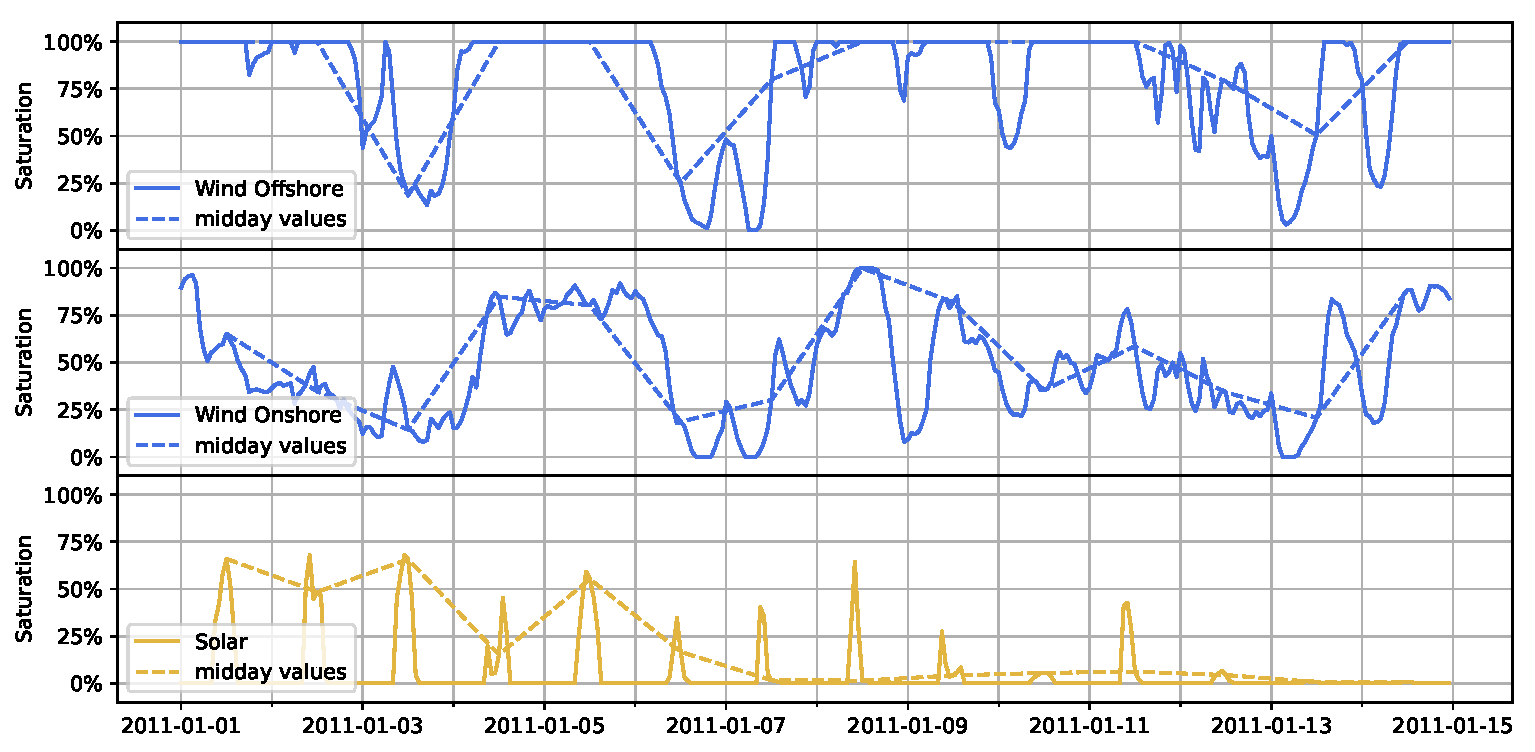
\includegraphics[width=\textwidth]{img/genseries270jan.pdf}
    \caption{Renewable generation capacity at bus \emph{`Emden-Borßum'} during the first two weeks of January. A dashed line is drawn through all midday (12:00) values for later reference.}\label{fig:genseries270jan}
\end{figure}

We can see a clear correlation between offshore and onshore wind generation. This should come as no surprise, since the offshore wind park and the onshore wind turbines are in close proximity (both are close to \emph{`Emden-Borßum'}), and are therefore exposed to similar weather. We also notice that the offshore generation is often \emph{saturated}: the saturation is capped at $100\si{\percent}$. When examining this phenomenon for all five offshore generators, we find that, on average, offshore generation was saturated ($\geq 95 \si{\percent}$) during $34\si{\percent}$ (SD $8\si{\percent}$) of measured hours. Saturation is rare for onshore wind generation ($2.4\si{\percent}$, SD $1.6\si{\percent}$) and solar generation ($< 0.5\si{\percent}$ for all buses). This saturation might be an artefact of the used dataset.

In the solar generation series, one can clearly identify the daylight hours, which span about 8 hours in January.\footnote{In Germany. For comparison: a day is 16 hours long in July.} We see some sunny days (day 3, for example), overcast days (day 5), and cloudy days (the last two days). The low efficiency on cloudy days might be a little extreme, but the generation series look to be realistic in general. The solar and wind series also agree with historical weather data.

\towrite{Geographical correlation}


\section{LPF}
As part of the OPF results calculated using \texttt{PyPSA}, we also get the \emph{line currents} for each hour. When calculating the currents using the LPF (applied to the power injections given in the OPF results), we find results that are very similar, but not exactly the same. The largest \emph{relative} discrepancies take place on lines with the smallest thresholds. Figure \ref{fig:lineflowcorrelationpypsa} shows the current of each line at 11:00, as given by the OPF results, and calculated using the LPF. It looks like these errors are not the result of a \textit{systematic} error in the calculation of the LPF (the LPF is using the same line impedances, for example), and we assume that the result given by \texttt{PyPSA} is \emph{more accurate}. More importantly: the line flows given by \texttt{PyPSA} are on the edge of the feasibility region, giving us the kind of critically loaded state that we are interested in. The result of applying the LPF overestimates the current through some lines, beyond the feasibility limit of the OPF.

This discrepancy needs to be investigated further,\footnote{By studying the source code of \texttt{PyPSA} in more detail, for example.} but for now, we will continue our analysis by adding this discrepancy as \emph{error-correction term} to the LPF:
\[
\LPF_{new} : \quad\mat{p} \quad\mapsto\quad \LPF_{old}(\mat{p}) \quad +\quad (\mat{f}_{\texttt{PyPSA}} - \LPF_{old}(\mat{p}_{nom})).
\]
where $\mat{f}_{\texttt{PyPSA}}$ is the nominal flow given in the OPF results, and $\mat{p}_{nom}$ is the injection found by the OPF.
\begin{figure}
    \centering
    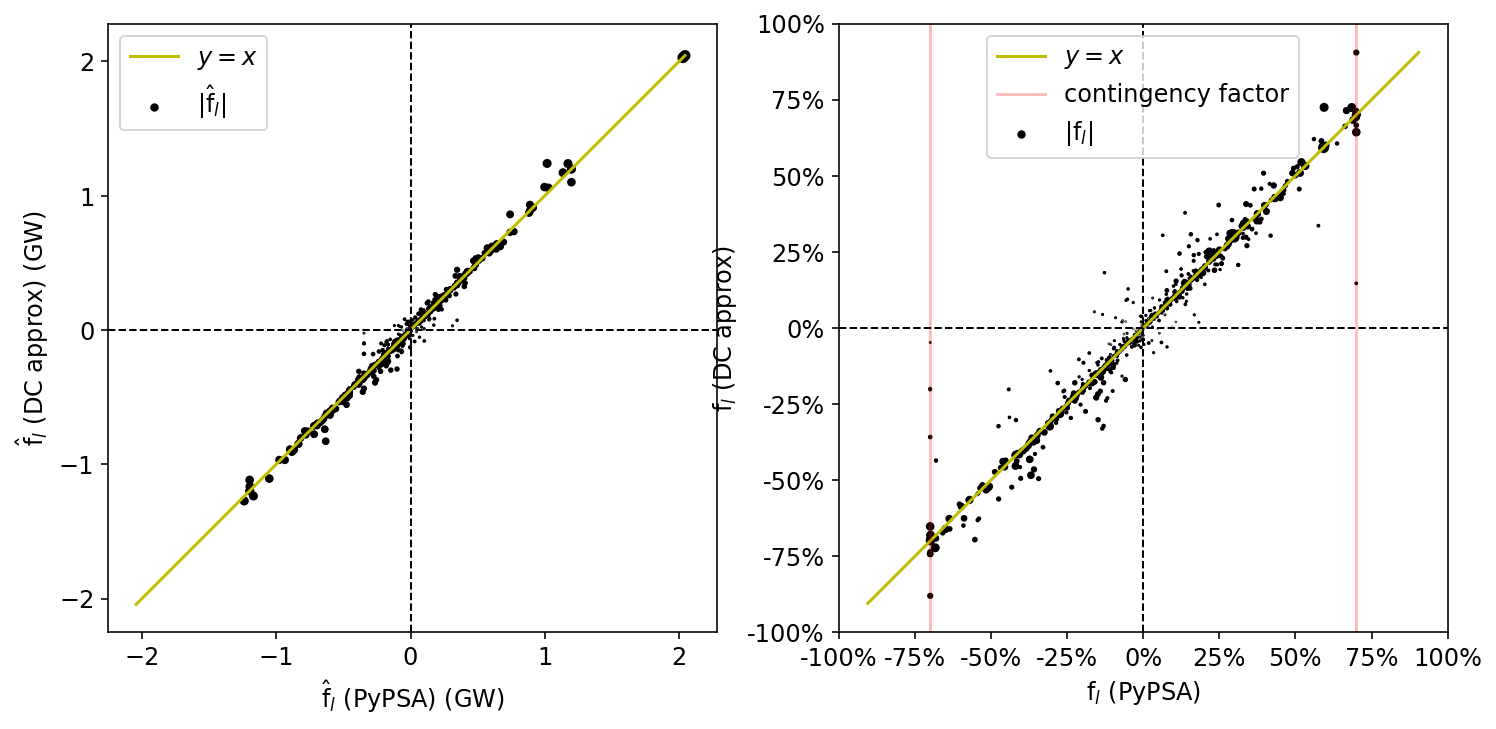
\includegraphics[width=\textwidth]{img/lineflowcorr.png}
    \caption{PLACEHOLDER: Line flow (left) and saturation (right) computed using LPF and (non-linear) PF.}
    \label{fig:lineflowcorrelationpypsa}
\end{figure}



\section{Stochastic power injection}
We model the power injection as a \emph{stochastic variable}. In particular, we will assume that the power injection is (multivariate) normally distributed, and we can use historical generation series to estimate this distribution. 



More generally, assuming the power injection captures the \emph{general uncertainty} of the exact amount of power injected during the 

Besides its useful mathematical properties, the normal distribution is a natural choice for modelling the `noise' of injected power, as each bus is the \emph{accumulation of all generators and loads} connected to the bus. When their individual contributions are \emph{random} (but not necessarily normally distributed), their combined effect will resemble a normal distribution by the Central Limit Theorem. 

Of course, the Central Limit Theorem can only be applied to individual contributions that are \emph{independently} distributed, which is not the case when studying renewable generation. For example, the amount of solar power generated at a bus is the sum of power generated by all individual solar panels in the region, but their fluctuations are \emph{highly correlated}; not independent.

\subsection{Generation forecast}
Grid operators use \emph{forecasting models} to predict the amount of stochastic power generated in the near future to guide their decisions. Advanced models use precise weather forecasts, and extrapolate the expected amount of stochastic generation. A cruder method is to simply look at past generation values of a single bus to predict future generation. We will discuss two models that use this latter method: the \emph{ARMA model} and the \emph{persistent forecast model}.

No forecast can be completely accurate: the real power injection will differ from the predicted injection by some error. This is where the \emph{stochastic} part of our model becomes useful: \textbf{we model this error to be normally distributed}. As covariance matrix, \cite{Nesti2018emergentfailures} propose \emph{computing the error values for historical generation series}, and using their covariances as covariance matrix for the normally distributed (future) errors.

This way, the normal distribution captures only correlations in forecast errors, and not correlations in the generation series themselves. This is desirable, because line overloads do not necessarily occur because of large or small amounts of stochastic generation: as long as this amount is known \emph{ahead of time}, the grid operator will adjust the generator configuration to maintain a feasible state. Rather, line overloads may occur when there is a large, sudden fluctuation in stochastic generation that was not predicted by the grid operator (\ie a large forecast error.)

While we do not know what forecast models are used by the grid operators in Germany, they are certainly beyond the scope of this thesis. So instead of using realistic forecast models, we use a \emph{placeholder model}. \cite{Nesti2018emergentfailures} use two ARMA models for this purpose (one for wind, one for solar). An attempt to recreate their results is described in Section \ref{sec:armamodel}. 

Because of the possibly unnecessary complexity of these ARMA models, we introduce a simpler model: the \emph{persistent forecast model}, which predicts the future generation to be equal to the present generation. Although this model does not necessarily provide an accurate forecast, it is sufficient for the purpose of a placeholder model.

\subsection{ARMA model}\label{sec:armamodel}
\towrite{TODO}

\subsubsection{Computing ARMA fits}\label{arimamod}
Following \cite{Nesti2018emergentfailures}, the ARMA models were fitted to the first month of solar and wind generation series using the \texttt{arima} method in \texttt{R}. This produced a result for all wind series.

Unfortunately, for the solar series, the \texttt{arima} method failed to fit an ARMA model for 104 of the 489 buses, reflecting the hypothesis that these series are poorly modelled by an ARMA series. To recreate the results of \cite{Nesti2018emergentfailures}, it is crucial that a model can be fitted for \emph{every} bus. Therefore, a modified method is required.

By the default, the \texttt{arima} method operates in two steps. First, a so-called Conditional-Sum-of-Squares (CSS) method is used as initial guess for the ARMA coefficients. Then, the coefficient \emph{likelihood} function is maximised with the Nelder-Mead optimisation method, using the CSS result as initial value.

In our case, the CSS method often finds initial values that are \emph{non-stationary}.\todo{define?} A possible reason is that solar generation is exactly zero during nighttime, which lasts for up to 16 consecutive hours.\footnote{In reality, solar generation is never \emph{exactly} zero, even after sunset, because solar panels also receive ambient light. This is not included in the (artificial) dataset.
%Ambient light includes sunlight scattered by the atmosphere (\eg 3 hours of twilight in January), artificial light
%TODO
}
To resolve this issue, we use an optimisation method that works well without specifying an initial value: it should find the \emph{global} maximum independently. The Simulated Annealing (SANN) algorithm included in \texttt{R} is such a method, and was chosen for this analysis.

With SANN as optimisation method, \texttt{arima} was able to fit solar models for 484 out of 489 buses. For the remaining 5 buses, a second technique is applied: to accommodate for the long periods of zero generation, a small amount of uniform noise is superimposed on the generation series. Initially, the noise magnitude is set to 1\% of the solar capacity of the bus. This percentage is increased iteratively, until the modified method is able to fit a solar model. In fact, 1\% noise proved sufficient for the remaining 5 buses in January, and no more than 2\% noise was needed for any bus in the remaining months.

The modified method described in this section was used to fit solar and wind models to each bus of the network, for each month of 2011. Table \ref{tab:arimafitstats} lists the number of buses that can be analysed using the default and modified methods, showing the poor performance of the default for solar series, especially during the months of summer.
\tocite{Belisle 1992, zie \texttt{optim} docs}

\citet{Nesti2018emergentfailures} do not mention such problems (nor techniques to solve them). Because the same dataset, processing, programming language and method was used in this analysis, it is likely that they have also encountered and solved these problems, possibly in the same manner.
\towrite{discuss other possible techniques: warm start, intercept}

\subsubsection{Runtime}
The default implementation has an estimated (single-core) runtime of 101 hours (4.2 days) when all 12 months are analysed, although only 78\% of fits are successful using this method.

The modified version is able to fit all generation series successfully. The use of this more computationally expensive method increases the runtime to an estimated 224 hours (9.4 days). Because of the long runtime, fits were computed in parallel on a 40-core machine\footnote{Specifications: two \textit{Intel Xeon E5 2630L v4} 10-core processors @2GHz with hyperthreading; 64GB RAM. CPU time was used as estimate for single-core runtime.}, provided by the IT department of the Radboud University.\footnote{Thank you!} This reduced the total runtime down to 7 hours. The results are publicly available at the GitHub repository.

\subsection{Persistent forecast model}
\towrite{In plaats van een ARMA model gebruiken we het model $X_t = X_{t-1}$, en we bekijken de covarianties van fouten volgens deze 'voorspelling'. De reeks van fouten is dan simpelweg de verschilrij.

Voor het windmodel komt dit eigenlijk sterk overeen met het gefitte ARMA-model, ik heb hier veel plotjes over.}
\subsection{Bus covariance matrix}
Using each method, we find covariance matrices for solar generation and wind generation. Following \cite{Nesti2018emergentfailures}, we use these matrices to construct the two \emph{bus covariance matrices}: 
\[
\mat{\Sigma}_{\text{day}} = \mat{\Sigma}_{\text{wind}} + \mat{\Sigma}_{\text{solar}} \qquad \mat{\Sigma}_{\text{night}} = \mat{\Sigma}_{\text{wind}}.
\]
\section{Stochastic line flows}
\towrite{Eigenlijk is er over de \emph{methode} hier niet veel te zeggen, dit is in het vorige hoofdstuk al gedaan. (Misschien hier naartoe verplaatsen? en het vorige hoofdstuk laten eindigen na de LPF-vergelijking) De resultaten staan in het volgende hoofdstuk.}

\subsection{Line failures}
\towrite{idem}

\section{Most likely power injection}
The most likely power injection, given the failure of a line, can be computed directly using Theorem~\ref{thm:mostlikelyinjection}. This method is numerically stable, even when the failure probability is, to numerical approximation, equal to $0$. Also, while the proof of Theorem~\ref{thm:mostlikelyinjection} uses (the existence of) the inverse of $\mat{\Sigma}_{\mat{p}}$, it is not required in the final expression.

When examining the result of this calculation for a number of lines, we found two problems with the final result, which are most prominent on stable lines (those with negligible overload probability).

\subsection{Non-zero net injection}
First, the most likely injection might not have zero sum. We can safely apply the matrix $\mat{F}$ to an injection $\mat{p}$ that does not have zero sum. Nevertheless, under our assumptions, $\mat{p}$ must have zero sum. As part of the DC approximation, we found that the power injection is the image of $\mat{L} = \mat{K}\diag(i\mat{\eta})\mat{K}^*$, applied to the vector of phase angles, $\mat{\theta}$ (Equation \ref{eq:approxnodeflowlineq}). From Theorem~\ref{thm:imageLPF} it then follows that the power injection should have zero sum.

Instead of concluding that our model, and the results that follow, are therefore entirely invalid, we will simply \emph{ignore this problem}. We do so with the same reasoning as \cite{Nesti2018emergentfailures}: in reality, the total power injection is never exactly of zero sum. As discussed in Section \ref{sec:loads}, turning any grid-connected device on or off will change the total injection. This does \emph{not} cause the power grid to `promptly vanish in a puff of logic', but rather, it physically causes a \emph{change of AC frequency}. This change in frequency is then measured by grid operators and generators, who react by changing their energy output to compensate for the change in frequency. This feedback loop is \emph{stable} \citep{VonMeier2006}, as long as frequency changes are small, and the demand can be met.\footnote{Note that this is a one-sentence simplification of the study of \define{grid stability}.}

The generators (or rather, the the buses that they are connected to) that respond to a change in AC frequency are called the \emph{slack buses}\index{slack bus} of the network, and they are chosen by the grid operator. In our discussion of the energy market (\ref{sec:energymarkey}), we assumed, for didactic simplicity, that a single generator is assigned to be the slack bus.

\cite{Nesti2018emergentfailures} assume, for mathematical simplicity, that all generators play this role, which is called \emph{distributive slack}. The individual amounts of change in generation is chosen such that the line flows after all generators have settled into a zero-sum are exactly equal to $\mat{F}\mat{p}^{init}$, where $\mat{p}^{init}$ is the initial, non-zero power injection. This redistributed injection is given by:
\[
\mat{p}^{slack} = \mat{K}\mat{F}\mat{p}^{init}.
\]
When $\mat{p}^{init}$ \emph{does} have zero sum, we find $\mat{p}^{slack} = \mat{p}^{init}$, since $\mat{F}$ is the right-inverse of $\mat{K}$, when restricted to the set of zero-sum injections.

\subsection{Unrealistic renewable fluctuations}
The second problem with the most likely injection is that it might not be realistic, simply because there are not enough solar panels and wind turbines to produce the predicted injection. A simple way to check this condition is to calculate the predicted increase in renewable generation at each node, and compare it to the installed capacity.

\towrite{In Nesti is duurzame opbrengst een som van stochasten, en dus kan de maximale capaciteit wel worden overschreden (de capaciteit is dan 'een schatting van een gemiddelde bovengrens' oid). We kunnen dus beter berekenen met hoeveel procent we de capaciteiten moeten rekken daarvoor. Verder is de data slechts een schatting van capaciteit.}

\section{Cascading line failures}\label{sec:cascades}
\towrite{precies wat je denkt: herdistributie bereken, lijnen weghalen, etc}

\towrite{misschien een beknopte samenvatting van het model aan het einde/begin van dit hoofdstuk?}
\end{document}
